\documentclass[12pt]{article}
\usepackage{amsmath}
\usepackage{amssymb}
\usepackage{graphicx}
\usepackage{subcaption}
\usepackage{cite}
\usepackage{hyperref}
\usepackage{float}

\title{Path Tracing Renderer Using Monte Carlo Methods}
\author{Silas Maughan}
\date{\today}

\begin{document}

\maketitle

\begin{abstract}
    This report presents a study on the implementation of a path tracing renderer using Monte Carlo methods to simulate realistic lighting in a 3D scene. Various sampling techniques and variance reduction methods are explored to enhance image quality and convergence speed. Experimental results demonstrate the effectiveness of these techniques in reducing noise and improving rendering efficiency. The report discusses the mathematical foundations, implementation details, and performance evaluations of different Monte Carlo sampling strategies and variance reduction techniques.
\end{abstract}

\tableofcontents

\section{Introduction}
\label{sec:intro}
Path tracing is a rendering technique used to create realistic images by simulating the way light interacts with objects in a scene. Unlike traditional ray tracing, which traces a single path of light from the eye to the light source, path tracing traces multiple light paths to account for complex interactions like reflection, refraction, and scattering. This report details the implementation of a path tracing renderer using Monte Carlo integration to approximate the rendering equation.

\section{Background and Related Work}
\label{sec:background}
\subsection{Monte Carlo Methods in Path Tracing}
Monte Carlo integration is a statistical technique used to approximate the rendering equation by randomly sampling light paths and averaging their contributions to pixel color. The rendering equation, formulated by Kajiya in 1986, is given by:

\begin{equation}
    L_o(\mathbf{x}, \omega_o) = L_e(\mathbf{x}, \omega_o) + \int_{\Omega} f_r(\mathbf{x}, \omega_i, \omega_o) L_i(\mathbf{x}, \omega_i) (\omega_i \cdot \mathbf{n}) \, d\omega_i
\end{equation}

where:
\begin{itemize}
    \item $L_o(\mathbf{x}, \omega_o)$ is the outgoing radiance at point $\mathbf{x}$ in direction $\omega_o$.
    \item $L_e(\mathbf{x}, \omega_o)$ is the emitted radiance at point $\mathbf{x}$ in direction $\omega_o$.
    \item $f_r(\mathbf{x}, \omega_i, \omega_o)$ is the bidirectional reflectance distribution function (BRDF) at point $\mathbf{x}$ for incoming direction $\omega_i$ and outgoing direction $\omega_o$.
    \item $L_i(\mathbf{x}, \omega_i)$ is the incoming radiance at point $\mathbf{x}$ from direction $\omega_i$.
    \item $\omega_i \cdot \mathbf{n}$ is the cosine of the angle between the incoming direction $\omega_i$ and the surface normal $\mathbf{n}$.
    \item $\Omega$ is the hemisphere above the point $\mathbf{x}$.
\end{itemize}

\subsection{Monte Carlo Integration}
Monte Carlo integration estimates an integral by averaging the function evaluated at randomly chosen points. The Monte Carlo estimator for the integral is:

\begin{equation}
    \hat{I} = \frac{1}{N} \sum_{i=1}^{N} f(\mathbf{x}_i)
\end{equation}

where $\hat{I}$ is the estimated integral, $N$ is the number of samples, and $f(\mathbf{x}_i)$ is the integrand evaluated at the $i$-th sample point $\mathbf{x}_i$. The variance of the estimator decreases as the number of samples increases, making this method particularly suitable for high-dimensional integrals like the rendering equation.

\subsection{Sampling Techniques}
Different sampling strategies affect the efficiency and quality of the rendered images. Uniform sampling, importance sampling, and stratified sampling are common techniques used in Monte Carlo integration for path tracing.

\textbf{Uniform Sampling:} Samples are taken uniformly across the domain. While simple to implement, this method can result in high variance and slow convergence.

\textbf{Importance Sampling:} Samples are drawn from a distribution that closely matches the integrand, reducing variance and improving convergence.

\textbf{Stratified Sampling:} The domain is divided into strata, and samples are taken from each stratum. This technique reduces variance by ensuring a more even coverage of the domain.

\subsection{Variance Reduction Techniques}
Variance reduction techniques aim to minimize the noise in the rendered image without significantly increasing the number of samples. These techniques include antithetic variates, control variates, and Russian roulette termination.

\textbf{Antithetic Variates:} Pairs of negatively correlated samples are used to reduce variance.

\textbf{Control Variates:} Known functions with calculable expected values are used to adjust the estimator, reducing variance.

\textbf{Russian Roulette Termination:} Paths are terminated probabilistically to balance the computational cost and variance reduction.

\subsection{Related Work}
Path tracing and Monte Carlo methods have been extensively studied in computer graphics. Key contributions include Kajiya's rendering equation, Veach's work on bidirectional path tracing, and various techniques for variance reduction and importance sampling.

\section{Methodology}
\label{sec:methodology}
\subsection{Scene Setup}
A basic 3D scene is created with simple geometric objects, a light source, and a camera. The scene includes objects like spheres and planes, and a point light source to illuminate the scene. The camera is positioned to capture the entire scene.

\subsection{Basic Ray Tracing Algorithm}
A basic ray tracing algorithm is implemented to handle the initial light path calculations. Rays are traced from the camera through each pixel and into the scene. The algorithm calculates intersections with objects, reflects or refracts rays as necessary, and accumulates the color contributions along the path.

\subsection{Monte Carlo Integration Framework}
The Monte Carlo integration framework is developed for the path tracing renderer. Light paths are traced stochastically, and their contributions are averaged to approximate the solution to the rendering equation. Specifically, the Monte Carlo estimator for the integral can be represented as:

\begin{equation}
    \hat{I} = \frac{1}{N} \sum_{i=1}^{N} f(\mathbf{x}_i)
\end{equation}

where $\hat{I}$ is the estimated integral, $N$ is the number of samples, and $f(\mathbf{x}_i)$ is the integrand evaluated at the $i$-th sample point $\mathbf{x}_i$.

\subsection{Diffuse Renderers}
Two diffuse rendering techniques have been implemented so far:

\textbf{Completely Diffuse:} In this technique, a random vector is generated from the hit point, resulting in completely uniform scattering rays.

\textbf{Lambertian Diffuse:} Here, a random vector from within a unit sphere at the hit point is added to the reflected normal, causing the rays to tend toward the normal direction.

% MENTION THE POINT OF IT, NOT SPEED BUT VISUAL FIDELITY
\begin{figure}[H]
    \centering
    \begin{subfigure}[b]{0.45\textwidth}
        \centering
        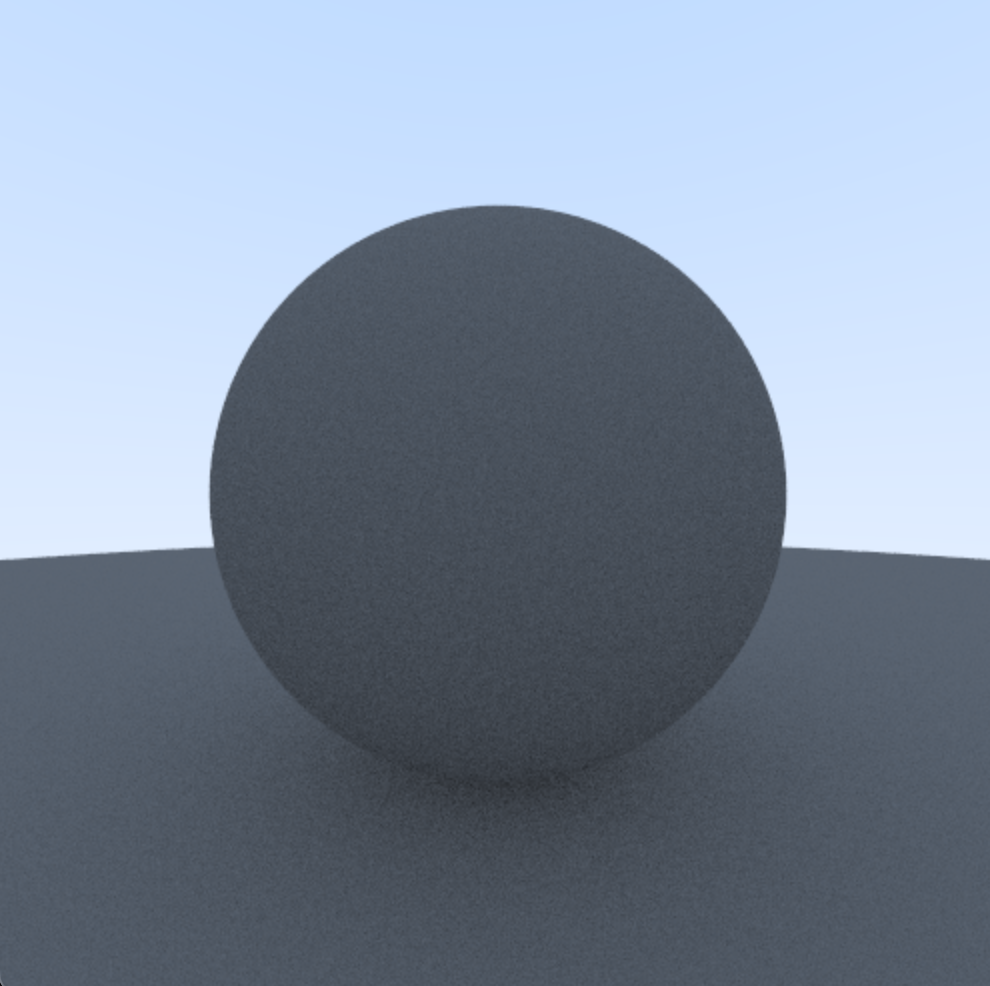
\includegraphics[width=\textwidth]{images/uniform_diffuse.png}
        \caption{Rendered image using Uniform Diffuse Renderer}
        \label{fig:completely_diffuse}
    \end{subfigure}
    \hfill
    \begin{subfigure}[b]{0.45\textwidth}
        \centering
        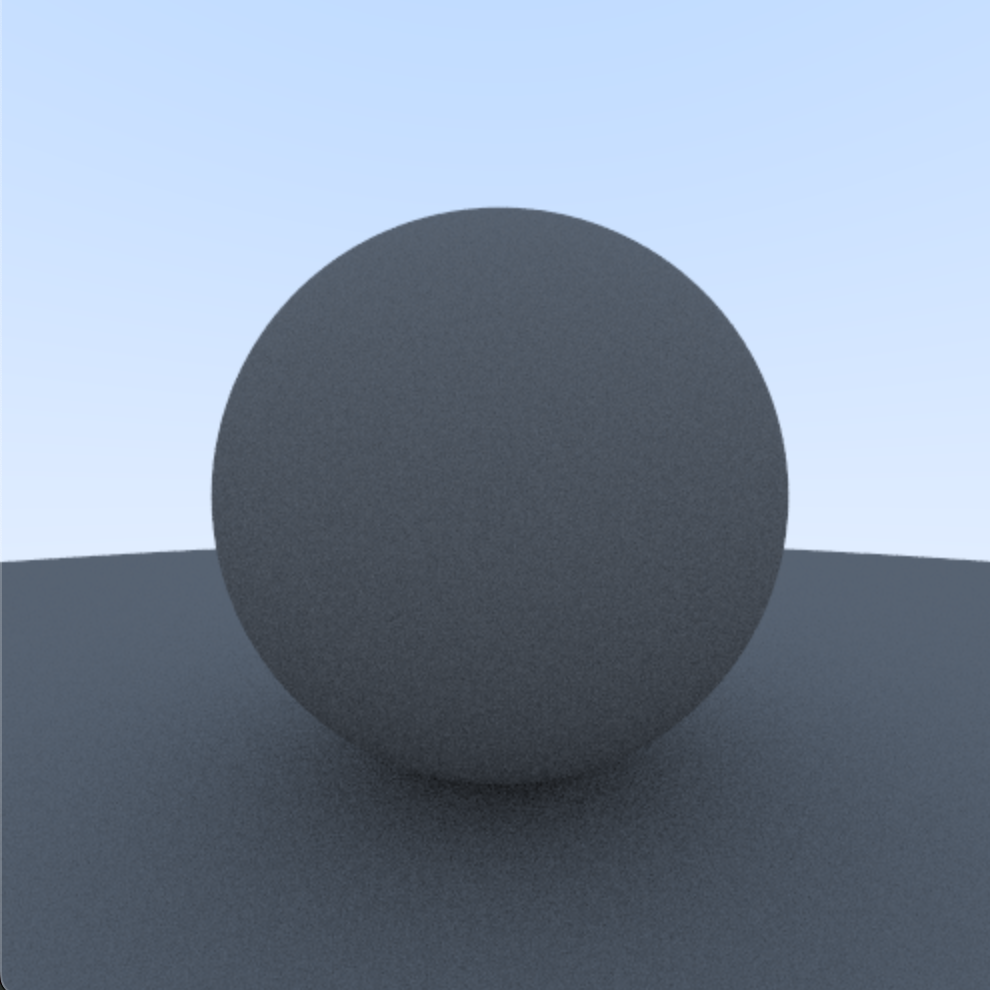
\includegraphics[width=\textwidth]{images/lambertian_diffuse.png}
        \caption{Rendered image using Lambertian Diffuse Renderer}
        \label{fig:lambertian_diffuse}
    \end{subfigure}
    \caption{Comparison of rendering techniques}
    \label{fig:rendering_comparison}
\end{figure}

\subsection{Sampling Techniques}
\subsubsection{Uniform Sampling}
Random samples are generated uniformly across the hemisphere above each intersection point. The contributions of these samples are averaged to estimate the pixel color.

\subsubsection{Importance Sampling}
Importance sampling is implemented by generating samples according to the distribution of the BRDF at each intersection point. This focuses sampling efforts on the most significant light paths, reducing variance. The estimator in importance sampling is given by:

\begin{equation}
    \hat{I} = \frac{1}{N} \sum_{i=1}^{N} \frac{f(\mathbf{x}_i)}{p(\mathbf{x}_i)}
\end{equation}

where $p(\mathbf{x}_i)$ is the probability density function used for sampling.

\subsubsection{Stratified Sampling}
Stratified sampling is implemented by dividing the hemisphere into strata and sampling within each stratum. This ensures a more even coverage of the hemisphere and reduces variance compared to uniform sampling. The variance of the estimator in stratified sampling can be expressed as:

\begin{equation}
    \text{Var}(\hat{I}) = \frac{1}{N} \sum_{i=1}^{N} \text{Var}(f(\mathbf{x}_i) - \mathbb{E}[f(\mathbf{x}_i)])
\end{equation}

\subsection{Variance Reduction Techniques}
Variance reduction techniques such as antithetic variates, control variates, and Russian roulette termination are introduced to enhance image quality.

\textbf{Antithetic Variates:} Pairs of negatively correlated samples are used to reduce variance. If $\mathbf{X}$ and $\mathbf{X}'$ are antithetic pairs, then the estimator becomes:

\begin{equation}
    \hat{I} = \frac{1}{2N} \sum_{i=1}^{N} \left( f(\mathbf{X}_i) + f(\mathbf{X}'_i) \right)
\end{equation}

\textbf{Control Variates:} Known functions with calculable expected values are used to adjust the estimator, reducing variance. If $h(\mathbf{x})$ is a control variate with known expected value $\mathbb{E}[h(\mathbf{x})]$, the estimator is:

\begin{equation}
    \hat{I} = \frac{1}{N} \sum_{i=1}^{N} \left( f(\mathbf{x}_i) + c (h(\mathbf{x}_i) - \mathbb{E}[h(\mathbf{x})]) \right)
\end{equation}

\textbf{Russian Roulette Termination:} Paths are terminated probabilistically to balance the computational cost and variance reduction. The probability of termination is denoted by $p$, and the estimator becomes:

\begin{equation}
    \hat{I} = \frac{1}{N} \sum_{i=1}^{N} \frac{f(\mathbf{x}_i)}{1 - p}
\end{equation}

\section{Results and Analysis}
\label{sec:results-analysis}
\subsection{Current Progress}
The following components have been completed:
\begin{itemize}
    \item Scene setup with simple objects (spheres) and a camera.
    \item Basic ray tracing algorithm.
    \item Implementation of Monte Carlo integration framework.
    \item Implementation of random sampling for light paths.
    \item Calculation of pixel colors based on average contributions from sampled paths.
    \item Completely diffuse renderer.
    \item Lambertian diffuse renderer.
\end{itemize}

\subsection{Future Visualizations}
Figures \ref{fig:completely_diffuse} and \ref{fig:lambertian_diffuse} show the rendered images using the completely diffuse renderer and the Lambertian diffuse renderer, respectively. Future visualizations will include results from uniform sampling, importance sampling, and stratified sampling techniques.

\section{Experiments and Results}
\label{sec:experiments}
\subsection{Image Quality and Convergence Analysis}
The impact of each sampling method on image quality and convergence will be visualized and analyzed. Uniform sampling, importance sampling, and stratified sampling will be compared in terms of the noise level and convergence speed.

\begin{figure}[h]
    \centering
    %\includegraphics[width=0.8\textwidth]{uniform_sampling.png}
    \caption{Rendered image using Uniform Sampling}
    \label{fig:uniform_sampling}
\end{figure}

\begin{figure}[h]
    \centering
    %\includegraphics[width=0.8\textwidth]{importance_sampling.png}
    \caption{Rendered image using Importance Sampling}
    \label{fig:importance_sampling}
\end{figure}

\begin{figure}[h]
    \centering
    %\includegraphics[width=0.8\textwidth]{stratified_sampling.png}
    \caption{Rendered image using Stratified Sampling}
    \label{fig:stratified_sampling}
\end{figure}

\subsection{Noise Level and Performance Comparison}
Noise levels and performance improvements with different variance reduction techniques will be measured and compared. Figures \ref{fig:antithetic_variates}, \ref{fig:control_variates}, and \ref{fig:russian_roulette} will demonstrate the noise reduction achieved by each variance reduction technique.

\begin{figure}[h]
    \centering
    %\includegraphics[width=0.8\textwidth]{antithetic_variates.png}
    \caption{Rendered image using Antithetic Variates}
    \label{fig:antithetic_variates}
\end{figure}

\begin{figure}[h]
    \centering
    %\includegraphics[width=0.8\textwidth]{control_variates.png}
    \caption{Rendered image using Control Variates}
    \label{fig:control_variates}
\end{figure}

\begin{figure}[h]
    \centering
    %\includegraphics[width=0.8\textwidth]{russian_roulette.png}
    \caption{Rendered image using Russian Roulette Termination}
    \label{fig:russian_roulette}
\end{figure}

\subsection{Convergence Rate Study}
Experiments will be conducted to study the convergence rate of the path tracer. The number of samples per pixel will be varied, and the resulting image quality will be evaluated to understand the relationship between the number of samples and image accuracy. Figure \ref{fig:convergence_rate} will show the convergence rate for different sampling techniques.

\begin{figure}[h]
    \centering
    %\includegraphics[width=0.8\textwidth]{convergence_rate.png}
    \caption{Convergence rate for different sampling techniques}
    \label{fig:convergence_rate}
\end{figure}

\section{Discussion}
\label{sec:discussion}
\subsection{Statistical Analysis}
Statistical analysis will be used to demonstrate the effects of different sampling techniques and variance reduction methods on image quality. The variance and bias of each method will be discussed, and the effectiveness of each technique in reducing noise and improving convergence will be evaluated.

\subsection{Number of Samples and Image Accuracy}
The analysis will show how the number of samples affects image accuracy and convergence. More samples generally lead to higher accuracy but at a higher computational cost. The trade-offs between sample count, image quality, and rendering time will be discussed. The efficiency of various variance reduction techniques will be evaluated to determine their practicality in different rendering scenarios.

\section{Conclusion}
\label{sec:conclusion}
The study demonstrates that Monte Carlo methods are effective for path tracing and realistic image synthesis. Importance sampling and stratified sampling significantly improve image quality and convergence speed compared to uniform sampling. Variance reduction techniques further enhance the rendering efficiency by reducing noise. Future work could explore more advanced sampling strategies and real-time rendering optimizations. The implementation of these techniques in a practical renderer highlights the importance of statistical methods in achieving high-quality, efficient rendering solutions.

\section{Future Work}
\label{sec:future-work}
The following tasks are planned for further development:
\begin{itemize}
    \item Implementation and comparison of uniform sampling, importance sampling, and stratified sampling.
    \item Visualization and analysis of the impact of each sampling method on image quality and convergence.
    \item Addition of variance reduction techniques to the path tracer.
    \item Measurement and comparison of noise levels and performance improvements.
    \item Conducting experiments to study the convergence rate of the path tracer.
    \item Using statistical analysis to demonstrate how the number of samples affects image accuracy.
\end{itemize}

\section{References}
\label{sec:references}
\bibliographystyle{plain}
\bibliography{references}

\end{document}